\chapter{Tensor-based Discriminative Sensing for Fraud Detection}
\label{ch:4_tensor_dl}

\begin{quotation}[]{Paulo Freire}
No one knows it all. No one is ignorant of everything. We all know something. We are all ignorant of something.
\end{quotation}

% \section{Introduction}
% Compressed Sensing | Dictionary Learning | Multidimensional data | Tensor DL and Separable dictionaries

Compressed Sensing (CS) aims to obtain the most relevant information of a dataset, what makes it useful for compression, signal reconstruction, image processing and classification, such as in sparce representation classification (SRC) problems. 

Dictionary learning is related to CS but seeks to obtain compact and meaningful signal representations, known as dictionary, from learning algorithms or models. DL is a signal processing technique for sparse representation of signals as basis vectors, learning the representations from training data, as dictionaries. DL is based on the principle that some observations can be described by a sparse subset of atoms taken from a redundant dictionary, which represents the causes of some observations of the world. The sparse representation in terms of such dictionaries has attracted increased interest for compressive sensing and for solving problems such as denoising, compression, image processing, data decomposition, feature extraction and classification, when the learning includes a class separability criteria in the objective function \cite{tosic2011dictionary, zhang2010discriminative, zhu2016coupled,ravishankar2011mr}. 

There are two major approaches for DL. First is the analytic approach, in which Discrete Cosine Transform basis, wavelets, curvelets and other nonadaptive functions are used as atoms to construct the dictionaries. Second is the learning-based approaches, such as the unsupervised learning for dictionary construction [9] and the online dictionary learning [11], [10], which use machine learning methods to construct the dictionary. 

In the analytic approach, some pre-defined functions are used to construct the dictionary. Curvelets [24], which tracks the shape of the discontinuity set, offers efficient and near-optimal representation of smooth objects. Shearlets [25], which is obtained from dilations, action of translations and shear transformations, has nice geometric properties and mathematical properties for image representation. Bandelets [26], which specifies the geometry as a vector field, is de-signed to improve the image compression and noise reduction performance. 

In the learning-based approach, machine learning methods are used to construct the dictionary from the training data. The least square error is used by the method of the optimal directions (MOD) [27] to update the dictionary iteratively. While analytic dictionaries permit to capture the global structure of a signal and allow a fast implementation, learned dictionaries often perform better in applications as they are more adapted to the considered class of signals.

In some applications, the data and its dictionary are multidimensional, e.g., when estimating jointly behavior of users in social networks. Computing tensor decompositions of multi-way datasets is particularly useful to extract hidden patterns and structure in multidimensional data analytics problems \cite{kolda2009tensor}. Tensor-based algorithms for DL can improve the performance for cases of multidimensional and separable data, regarding the dictionary identification rating, the required number of training samples and iterations for the optimization problem \cite{roemer2014tensor}. 

In imagery, the numerical burden for (i) learning a dictionary and for (ii) employing the dictionary for reconstruction tasks only allows to deal with relatively small image patches that only capture local image information. Separable dictionaries aims at overcoming these drawbacks by allowing a separable structure on the dictionary throughout the learning process. On the one hand, this permits larger patch-sizes for the learning phase, on the other hand, the dictionary is applied efficiently in reconstruction tasks. 

Multidimensional parameter estimation and learning multidimensional separable dictionaries are growing research problems. The crucial idea about separable dictionaries is to allow the dictionary to have a separable structure, where separable means that the dictionary $\textbf{D}$ is given by the Kronecker product of two smaller dictionaries $\boldsymbol{A}^{(1)} \in \mathbb{R}^{h \times a}$ and $\boldsymbol{A}^{(2)} \in \mathbb{R}^{w \times b}$, for example. Roemer \emph{et al.} \cite{roemer2014tensor} show that the multidimensional dictionary estimation problem can be efficiently formulated in terms of tensors, and that their results outperform existing schemes by exploiting the multilinear structure of the problem.

Considering that big data problems require techniques to deal with multidimensional data in order to make sense of strucutre and relationship of many dimensions, and also considering that a key challenge to use sparse coding and dictionary learning for classification is how to find proper dictionaries and coefficients that highligh discriminative structure and relationships of one dataset, this work propose a tensor-based DL for fraud detection from imbalanced data, in order to apply the tensor deconposition for DL methods to evidentiate the discriminative sensing of a fraud detection dataset. 

This chapter is organized as follows. Section \ref{sec:4_motivation} presents one experiment and results that motivate the proposed work. In Section \ref{sec:4_relatedworks}, related works are discussed. Section \ref{sec:4_datamodel} presents the data model and the evaluated datasets. Section \ref{sec:4_proposal} describes the proposed approach for for fraud detecton from mobile money transacion. Section \ref{sec:2_experimentalresults} discusses the experimental validation and presents the results, and Section \ref{sec:4_conclusion} draws the conclusions and the suggestions for future work.


\section{Motivation}
\label{sec:4_motivation}

Existing DL schemes can be applied to multidimensional analysis and obtain valuable results. However, the performance of tensor-based algorithms for recovering of a known separable dictionary outperform existing schemes when dealing with growing multidimensional datasets.

Considering that DL aims to obtain meaningful dictionaries, it is possible to evaluate DL algorithms by their performance to generate dictionaries that better represent one target data. Therefore, we can compare DL algorithms regarding recovering of a known dictionary. We conduct a evaluation of tensor-based DL algorithms for recovering a known dictionary in order to analyze the gains of tensor-based approaches in comparison to well known algorithms.

\subsection{Data Model and Experiments}
\label{sec:4_motivation_datamodel}

Consider a generic sparse recovery problem of the following form

\begin{equation}\label{eq:4_eq01}
	\boldsymbol{X} = \boldsymbol{A} \cdot \boldsymbol{S} + \boldsymbol{W},
\end{equation}

where $\boldsymbol{X} \in \mathbb{C}^{M \times T}$ represents $T$ consecutive observations from $M$ features, $\boldsymbol{A} \in \mathbb{C}^{M \times N}$ is the overcomplete dictionary where $N \ll T$, $\boldsymbol{S} \in \mathbb{C}^{N \times T}$ represents the sparse coefficient matrix, $\boldsymbol{W} \in \mathbb{C}^{M \times T}$ is the additive noise, and $M < N < T$.

Consider a sparse recovery problem for a separable 2-D dictionary that we can write as

\begin{equation}\label{eq:4_eq02}
	\boldsymbol{X} = (\boldsymbol{A}^{(1)} \otimes \boldsymbol{A}^{(2)}) \cdot \boldsymbol{S} + \boldsymbol{W},
\end{equation}

where $\boldsymbol{A} = (\boldsymbol{A}^{(1)} \otimes \boldsymbol{A}^{(2)})$, $\boldsymbol{A}^{(1)} \in \mathbb{C}^{M_1 \times N_1}$, $\boldsymbol{A}^{(2)} \in \mathbb{C}^{M_2 \times N_2}$, $M = M_1 \times M_2$, and $N = N_1 \times N_2$.

In order to evaluate tensor-based DL algorithms for recovering a known dictionary, we generate two random dictionaries $\boldsymbol{A}^{(1)}$ and $\boldsymbol{A}^{(2)}$ from an i.i.d. zero mean Gaussian random process, and calculate the dictionary $\boldsymbol{A}$ through the Kronecker product, according to 

\begin{equation}\label{eq:4_eq03}
	\boldsymbol{A} = (\boldsymbol{A}^{(1)} \otimes \boldsymbol{A}^{(2)}).
\end{equation}

Therefore, $\boldsymbol{A}$ is the known dictionary that shall be used for recovery evaluation. 

Subsequently, we generate a synthetic data set $\boldsymbol{X}$ using the given dictionary $\boldsymbol{A}$, according to Equation \ref{eq:4_eq01}, where $\boldsymbol{S}$ is a random sparse coefficient matrix for what we assume that each column has $K = 5$ non-zero entries, and $\boldsymbol{W}$ is the additive white gaussian noise. Thus, we estimate the initial $\boldsymbol{\hat{A}}$ dictionary from a normalized subset of $\boldsymbol{X}$ and make the dictionary separable decomposing the approximation of $\boldsymbol{\hat{A}}$ and generating $\boldsymbol{\hat{A}}^{(1)}$ and $\boldsymbol{\hat{A}}^{(2)}$ according to \cite{van1993approximation}. Afterward, we update $\boldsymbol{\hat{A}}$ through 

\begin{equation}\label{eq:4_eq04}
	\boldsymbol{\hat{A}} = (\boldsymbol{\hat{A}}^{(1)} \otimes \boldsymbol{\hat{A}}^{(2)}),
\end{equation}

and use it for DL experiments using MOD \cite{engan1999method}, K-SVD \cite{aharon2006rm}, RLS-DLA \cite{skretting2010recursive}, T-MOD \cite{roemer2014tensor} and K-HOSVD \cite{roemer2014tensor}. Due to its low computational complexity, we employ the Orthogonal Matching Pursuit (OMP) algorithm\cite{davis1997adaptive} for the sparse recovery stage in all the dictionary learning algorithms, assuming that K is known. However, other solver for sparse recovery can be used, such as Basis Pursuit \cite{chen2001atomic}, the LASSO algorithm \cite{tibshirani1996regression} or greedy \cite{davis1997adaptive}.

The final estimated dictionaries $\boldsymbol{\hat{A}}$ recovered by each DL algorithm are compared to the known dictionary $\boldsymbol{A}$, through a measure of the distance between two dictionaries. The recovered dictionary is then compared to the known dictionary, by using the angle between a known atom and a recovered atom as a distance measure. The number of identified atoms is computed by comparing these angles to a limit of $\beta_{lim} = 8.11$ degrees, that corresponds to the case where the inner product of the two compared atoms is equal to 0.99, and where each atom has 2-norm equal to 1.

For this experiments we adopt an additive noise with $snr = 20$ and 100 iterations for dictionary learning. All experiments run 100 trials in order to obtain confident results.

This evaluation extends Roemer \emph{et al.} \cite{roemer2014tensor} including RLS-DLA for comparison, and for adding the evaluation of the degree distribution for atom identification and the evaluation of the atom identification according to the dictionary size variation. Additionally, we conduct a experimental evaluation, while Roemer \emph{et al.} \cite{roemer2014tensor} presents numerical results obtained via Monte Carlo simulations.


\subsection{Results}
\label{sec:4_motivation_results}

Figures \ref{fig:fig1} and \ref{fig:fig2} show the evaluation of tensor-based (K-HOSVD \cite{roemer2014tensor} and T-MOD \cite{roemer2014tensor}) and traditional DL algorithms (RLS-DLA, K-SVD and MOD) for dictionary reconstruction of a multidimensional and separable data. These figures show the distribution of the cumulative atom identification over the degree rates.

Figure \ref{fig:fig1} presents the results for recovering a dictionary of $M=20$ and $N=50$. We see that the RLS-DLA method performs better than other methods, although T-MOD presents the best results for identification of up to 15 atoms of 50. It is possible to observe that T-MOD and K-HOSVD are better than MOD and K-SVD, and that the tensor-based methods outperforms MOD and K-SVD significantly for this experiment. Finally, Figure \ref{fig:fig1} shows that RLS-DLA recovered almost 40 atoms in $\beta_{lim} = 8.11$ degrees, while other methods present results lower results.

\begin{figure}[!htb]
	\centering 
	\includegraphics[width=10cm]{figures/5_20_2000_1000_100.eps}
	\caption{Cumulative atom identificatin per degree rates. $T=2000$, $M=20$, $N=50$}
	\label{fig:fig1}
\end{figure}

Figure \ref{fig:fig2} presents the results for recovering a dictionary of $M=80$ and $N=30$. It is possible to observe that the tensor-base methods outperform MOD, RLS-DLA and K-SVD in number of identified atoms and the required degrees for identification. Note that MOD performs quite silimar to RLS-DLA, while K-SVD is the worst evaluated case for this experiment. Considering the tensor-based methods, T-MOD outperforms K-HOSVD with higher atom identification over lower degrees. The experimental results verify that the tensor-based dictionary learning algorithms are able to identify more dictionary atoms when dealing with larger dictionaries and that they converge faster.

\begin{figure}[!htb]
	\centering 
	\includegraphics[width=10cm]{figures/5_20_2000_24000_100.eps}
	\caption{Cumulative atom identificatin per degree rates. $T=2000$, $M=80$, $N=30$}
	\label{fig:fig2}
\end{figure}

The results reveals that tensor-based algorithms can perform better for dictionary recovery problems when the dictionary size increases. Since dictionary learning and reconstruction error are usually used for sparce representation classification (SRC) problems, it is possible to supose that tensor-based algorithms can improve results of classification problems, as well as can extract hidden patterns and structure in multidimensional data analytics problems.

Recent developments in science and technology have enabled the growth and availability of raw data to occur at an explosive rate. This has created an immense opportunity for knowledge discovery and data engineering research to play an essential role in a wide range of applications from daily civilian life to national security. However, the high availability of raw data increases the challenges related to big data analytics and to imbalanced data, which corresponds to data sets exhibiting significant imbalances of classes or rare events of some classes. The fundamental issue with the imbalanced learning problem is the ability of imbalanced data to significantly compromise the performance of most standard learning algorithms

A key challenge to use SC and DL for classification is how to find proper dictionaries and coefficients that highligh discriminative structure and relationships of one dataset. Therefore, we introduce a tensor-based DL method for fraud detecton from unbalanced data. Specifically, we apply a sparse representation based classification (SRC) method through learning a tensor-based dictionary and evaluate the reconstruction error for fraud classification. 

In this chapter, we propose a tensor-based sparse representation and dictionary learning technique to analyze mobile money transactions in order to identify frauds. We propose to use tensor-based DL for learning fraudulent and legitimante data separetelly, and apply the learned dictionaries to reconstruct a test signal and classify it as fraud or ligitimate, according to the minimum reconstruction error measured by some metrics.


\section{Related Works}
\label{sec:4_relatedworks}

% Compressed Sensing | Dictionary Learning | Classification | Tensor-Based DL

Compressed sensing (also known as compressive sensing, compressive sampling, or sparse sampling) is a signal processing technique for efficiently acquiring and reconstructing a signal, by finding solutions to underdetermined linear systems. This is based on the principle that, through optimization, the sparsity of a signal can be exploited to recover it from far fewer samples than required by the Shannon-Nyquist sampling theorem. 

%There are two conditions under which recovery is possible.[1] The first one is sparsity which requires the signal to be sparse in some domain. The second one is incoherence which is applied through the isometric property which is sufficient for sparse signals.[2][3]. Around 2004, Emmanuel Candès, Terence Tao, and David Donoho proved that given knowledge about a signal's sparsity, the signal may be reconstructed with even fewer samples than the sampling theorem requires.[4][5] This idea is the basis of compressed sensing. 	https://www.wired.com/2008/03/engineers-test-highly-accurate-face-recognition/

Sparse coding is a sparse representation of one data in the form of a linear combination of basic elements. These elements are called atoms and they compose a dictionary. Dictionary learning is a representation learning method which aims at finding a sparse representation of the input data (also known as sparse coding) in the form of a linear combination of basic elements as well as those basic elements themselves. These elements are called atoms and they compose a dictionary. Atoms in the dictionary are not required to be orthogonal, and they may be an over-complete spanning set. This problem setup also allows the dimensionality of the signals being represented to be higher than the one of the signals being observed. The above two properties lead to having seemingly redundant atoms that allow multiple representations of the same signal but also provide an improvement in sparsity and flexibility of the representation.

One of the key principles of dictionary learning is that the dictionary has to be inferred from the input data. The emergence of sparse dictionary learning methods was stimulated by the fact that in signal processing one typically wants to represent the input data using as few components as possible. Before this approach the general practice was to use predefined dictionaries (such as fourier or wavelet transforms). However, in certain cases a dictionary that is trained to fit the input data can significantly improve the sparsity, which has applications in data decomposition, compression and analysis and has been used in the fields of image denoising and classification, video and audio processing. Sparsity and overcomplete dictionaries have immense applications in image compression, image fusion and inpainting.

MOD \cite{engan1999method} is a DL algorithm that is commonly used for extensions of Least-Squares (LS) type schemes, also known as iterative least squares dictionary learning algorithm (ILS-DLA) \cite{engan2007family}. MOD defines that if we know $\boldsymbol{S}$ in equation \ref{eq:4_eq01}, $\boldsymbol{A}$ can be estimated solving a linear LS problem. Additionally, knowing $\boldsymbol{A}$ we obtain $\boldsymbol{S}$ by solving a sparse recovery problem. MOD iterates between the two steps, starting with an initial guess of $\boldsymbol{A}$, denoted as $\hat{\boldsymbol{A}}$, which can be estimated, generated by previous dictionary learning or generated analitically. Despite - simplicity, the MOD algorithm has been criticized for its slow convergence, which is due to the fact that $\boldsymbol{A}$ and $\boldsymbol{S}$ are updated separately, which may lead to a slow convergence \cite{aharon2006rm}.

K-SVD \cite{aharon2006rm} is a generalization of the K-means algorithm for dictionary learning. After the sparse approximation step, the dictionary update is performed by sequentially updating each column of $\boldsymbol{A}$ using SVD to minimize the approximation error. The update step is hence a generalized K-means algorithm since each patch can be represented by multiple atoms and with different weights. In practice, dictionaries learned with K-SVD
have shown excellent performance in image denoising. 

Most DL algorithms update the dictionary after a batch of training vectors has been processed, usually using the whole set of training vectors as one batch. The training set is used iteratively to gradually improve the dictionary. The approach in RLS-DLA \cite{skretting2010recursive} is a continuous update of the dictionary as each training vector is being processed. The algorithm is based on recursive least squares (RLS) algorithm for adaptive filtering, what makes the algorithm less dependent on the initial dictionary and it improves both convergence properties of RLS-DLA as well as the representation ability of the resulting dictionary. 

Dimensionality reduction can first be achieved by selecting a subset of functions from a large, fixed dictionary that is used for the analysis of particular signals. These functions then determine a subspace of reduced dimension, where classification can be performed by computing the nearest neighbor points among the projected data. A simple method to build such a subspace consists in modifying the sparse approximation methods such that the objective function is augmented with a discrimination term that represents the separability properties of the projection subspace. This kind of approach typically tries to maximize the variance between the active atoms from $\boldsymbol{A}$ that represent signals in different classes. The reduced subspace used for classification is finally formed by the subset of atoms in $\boldsymbol{A}$ whose corresponding coefficients in $\boldsymbol{S}$ are nonzero. The subset selection problem can be interpreted as the inference step in the dictionary learning methods when the objective function is modified to include a discriminative term \cite{tosic2011dictionary}.

An important advantage of redundant dictionaries for classification is that signal analysis can be performed with functions that are likely to match the data characteristics in different classes of signals. Similarly to data approximation problems, data analysis applications can further benefit from dictionary learning methods. The previous section describes subspace selection methods from predefined dictionaries. DL algorithms can improve the classification performance, as it leads to a better adaptation of the dictionary by enforcing sparsity in the representation of data in the different classes. The atoms in a dictionary $\boldsymbol{A}$ that is computed with dictionary learning methods generally capture the most important constitutive components of the signals. They naturally permit to classify the data into the corresponding linear subspace. However, there is no guarantee that the subspace built on a learned dictionary $\boldsymbol{A}$ is truly optimal for classification, as it targets efficient representation but not necessarily class separability \cite{tosic2011dictionary}.

Dictionary learning methods should rather be modified so that they become simultaneously reconstructive and discriminative. The addition of a discriminative term into the dictionary learning algorithms requires supervision, where labels of training data are used to ensure that the data representation is sufficiently different in each class. It can be achieved by modifying the sparse coding step in the learning algorithms, so that it optimizes an objective function that favors the sparsest representation of a given signal and simultaneously the representation that is also the most different from the one of signals in other data classes. The supervised dictionary learning problem can be cast as a mixed formulation that minimizes the average value of the sparse approximation errors over different classes and also enforces discrimination between classes \cite{tosic2011dictionary}.

The use of one learned dictionary for all the data classes leads to a straightforward classification stage where the dictionary vectors and the coefficients in the signal representation are used directly to make classification decisions. Alternatively, one may want to improve the discrimination by building a distinctive projection subspace for each data class. Classification is then performed by selecting the subspace that is the nearest to the test signal, or equivalently the subspace that leads to the best representation of the test signal. A simple way to build adaptive dictionaries for each class is to use the signals in the training set for the class dictionary. Sparsity constraints are then rather applied within the classification process, where the sparsest representation of the test signal determines its class label \cite{tosic2011dictionary}.

Wright \emph{et al.} \cite{wright2009robust} have proposed a face recognition method that uses training face images as dictionaries and an $l_1$ sparse optimization method in the classification stage. The authors show that the recognition task can be successfully accomplished even using random features at first. Furthermore, the algorithm is robust to a certain amount of noise due to the sparsity constraints \cite{tosic2011dictionary}.

It is often preferable, however, to construct adapted dictionaries that can lead to an efficient classification process based on simple subspace projections. The construction of class dictionaries can be performed with learning methods where the sparse coding step in the iterative learning algorithms is modified, so that sparse coding is computed independently within each class. Such a sparse coding stage can be implemented by class-supervised versions of simultaneous pursuit algorithms \cite{tosic2011dictionary}.

Tensor data are typically highly structured, a perfect match for compressive sampling, so that the CS framework relaxes data acquisition requirements, enables compact storage, and facilitates data completion (i.e., inpainting of missing samples due to a faulty sensor or unreliable measurement) \cite{cichocki2015tensor}. Roemer \emph{et al.} \cite{roemer2014tensor} have proposed a tensor-based multidimensional extensions for MOD and K-SVD algorithms, which are respectivelly T-MOD and K-HOSVD, and show their improved performances numerically, for the dictionary reconstruction problem. 

Considering that tensor-based algorithms can perform better for dictionary recovery problems when the dictionary size increases, accordint to subsection \ref{sec:4_motivation_results}, we believe that tensor-based DL algorithms can improve the discriminative sensing for classification classification problems. Therefore, we propose use tensor-based DL for learning fraudulent and legitimante data separetelly, and apply the learned dictionaries to reconstruct a test signal and classify it as fraud or ligitimate, according to the minimum reconstruction error measured by some metrics

\section{Data Model}
\label{sec:4_datamodel}

% \subsection{Dataset}
% \label{sec:4_dataset}

We adopt a synthetic financial datasets for fraud detection\footnote{https://www.kaggle.com/ntnu-testimon/paysim1} in order to validate our proposal. This dataset is synthetically generated by  PaySim \cite{lopez2016paysim}, which is a financial simulator that simulates mobile money transactions based on an original dataset and provides a synthetic dataset as an approach to such a problem. PaySim uses aggregated data from the private dataset to generate a synthetic dataset that resembles the normal operation of transactions and injects malicious behaviour to later evaluate the performance of fraud detection methods. PaySim simulates mobile money transactions based on a sample of real transactions extracted from one month of financial logs from a mobile money service implemented in an African country. The original logs were provided by a multinational company

The selected dataset is composed by 9 features (variables) and 2.770.408 transactions (observations). It is also provided one lable that classifies each transaction as fraudulent or not. As the majority dataset of anomaly or fraud detection, the data is imbalanced, where the number of fraudulent transactions is 8.213 against 2.762.196 of normal transactions. Therefore, the fraud class represents 0,30 \% of the entire datased. 

For evaluation of the proposed classification approach we adopt a data splitting into training and test data, where the training data has 70 \% of the whole dataset. We denote the traning data as $X_r$ and the test data as $X_e$. The dataset can also be divided by normal and fraudulent transactions, where the normal train data is denoted as $X_r^o$, the fraud train data is denoted as $X_r^f$. The same notation of fraud, normal, train and test is applied to qualify $A$ and $S$.

% \subsection{Tensor-based Model}
% \label{sec:4_tensor_model}

% The Kronecker model (\ref{eq:4_eq02}) can be rewritten in an equivalent tensor form. Applying the algebraic rules for unfoldings of n-mode products \cite{roemer2014tensor} we can rewrite (\ref{eq:4_eq02}) into a "Tucker-2" decomposition, as

% \begin{equation}\label{eq:4_eq04}
% \boldsymbol{\mathcal{X}} = \boldsymbol{\mathcal{S}} \times_1 \boldsymbol{A}^{(1)} \times_2 \boldsymbol{A}^{(2)} + \boldsymbol{\mathcal{W}},
% \end{equation}

% where $\boldsymbol{\mathcal{X}} \in \mathbb{C}^{M_1 \times M_2 \times T}$, $\boldsymbol{\mathcal{S}} \in \mathbb{C}^{N_1 \times N_2 \times T}$, and $\boldsymbol{\mathcal{W}} \in \mathbb{C}^{M_1 \times M_2 \times T}$ are rearranged versions of the matrices $\boldsymbol{X}$, $\boldsymbol{S}$, and $\boldsymbol{W}$ such that $\boldsymbol{X} = [\boldsymbol{\mathcal{X}}]_{(3)}^T$, $\boldsymbol{S} = [\boldsymbol{\mathcal{S}}]_{(3)}^T$, and $\boldsymbol{W} = [\boldsymbol{\mathcal{W}}]_{(3)}^T$, respectively.

% We consider a randomly generated data in order to evaluate the proposed approach, where initially $\boldsymbol{A}^{(1)}$ and $\boldsymbol{A}^{(2)}$ are gaussian distributed and randomly generated, then the dictionary $\boldsymbol{A}$ is obtained. In order to be able to evaluate the dictionary reconstruction, the sparse data $\boldsymbol{\mathcal{X}}$ is generated from the dictionary $\boldsymbol{A}$, which is used for further comparisons. We adopt 20 as the signal-to-noise ratio (snr) and 5 as the sparseness factor of the data $\boldsymbol{\mathcal{X}}$. 

% The dictionary estimation is evaluated by applying the proposed approach to estimate the dictionary $\boldsymbol{A}$ from the sparse data $\boldsymbol{\mathcal{X}}$, according the selected number of sample training and iterations for the optimization problem.


\section{Tensor-based Sparce Representation Classification}
\label{sec:4_proposal}

We propose a Tensor-based Sparce Representation Classification approach to use tensor-based DL for learning fraudulent and legitimante data separetelly, and apply the learned dictionaries to reconstruct a test signal and classify it as fraud or ligitimate, according to the minimum reconstruction error measured by some metrics.

Our proposal requires supervision, where labels of training data are used to classify each transaction as fraud or normal. The first step is to split the training dataset into classes, as fraud or normal, and create respectively the data matrices $\boldsymbol{X}_r^f$ and $\boldsymbol{X}_r^o$. For each data matrix we compute the data normalization and subsequently the initial dictionaries $\boldsymbol{A}_r^f$ and $\boldsymbol{A}_r^o$. Afterward, we apply the dictionaries and the data matrices to the selected DL algorithms, in order to learn the best dictionaries $\boldsymbol{A}_r^f$ and $\boldsymbol{A}_r^o$ that respectivelly represents fraud and normal classes as basis vectors.

With the trainned dictionaries $\boldsymbol{A}_r^f$ and $\boldsymbol{A}_r^o$ and the test data $\boldsymbol{X}_e$ it is possible to process each transacion of $\boldsymbol{X}_e$, denoted as $\boldsymbol{x}_e^t$ where $t$ represents the transaction index, in order to compute its sparse coding from fraud and normal dictionaries, generating respectively $\boldsymbol{S}_e^f$ and $\boldsymbol{S}_e^o$. Subsequently, we compute the signal rescontruction as $\boldsymbol{x}_e^f = \boldsymbol{A}_r^f \cdot \boldsymbol{S}_e^f$ and $\boldsymbol{x}_e^o = \boldsymbol{A}_r^o \cdot \boldsymbol{S}_e^o$. 

Finally, we compare $\boldsymbol{x}_e^f$ and $\boldsymbol{x}_e^o$ to $\boldsymbol{x}_e^t$ in order to evaluate the reconstruction error to classify the transaction as fraud or normal according to the minimum reconstruction error from $\boldsymbol{x}_e^f$ and $\boldsymbol{x}_e^o$, respectivelly. We adopt the cosine similarity to compare the reconstructed signal to the original one. 


\section{Experiments}
\label{sec:4_experiments}

For data analysis of imbalanced classes it is usually applied a data undersample method, where an under sized sample is selected from the original datased, with similar amount of occurrences for each class of the data. This method is efficient for algorithm trainning, but it faces generalization problems when tries to classify new data. Therefore, we propose to evaluate the our proposal for under sampled data and for the complete dataset.

The Receiver Operating Characteristics (ROC) curve makes use of the proportion of two metrics: true positives rate (TPR) and false positives rate (FPR), which are defined as:

\begin{equation}\label{eq:4_eq04}
	TPR = \frac{TP}{Pc},
\end{equation}

\begin{equation}\label{eq:4_eq05}
	FPR = \frac{FP}{Nc},
\end{equation}

where $TP$ denotes true positive, $Pc$ is the total positive values, $FP$ denotes the false positive and $Nc$ the total negative values.

ROC curves are commonly used to present results for binary decision problems in machine learning. However, when dealing with highly skewed datasets, Precision-Recall (PR) curves give a more informative picture of an algorithm’s performance \cite{davis2006relationship, he2009learning}. The PR curve is defined by plotting Precision Rate (PR) over the Recall Rate (RR), which are defined as:

\begin{equation}\label{eq:4_eq06}
	PR = \frac{TP}{TP + FP},
\end{equation}

\begin{equation}\label{eq:4_eq07}
	RR = \frac{TP}{TP + FN}.
\end{equation}

PR curves exhibit a strong correspondence to ROC curves: A curve dominates in ROC space if and only if it dominates in PR space. However, an algorithm that optimizes the AUC in the ROC space is not guaranteed to optimize the AUC in PR space. Considering that our data is very imbalanced, with many more negatives than positives values, we adopt the averate precision recall for the classification evaluation

Logistic regression is the most common method used to model binary response data \cite{hilbe2011logistic}, it is useful for situations in where it is necessary to predict the presence or absence of a characteristic, with binary classification, such as in anomaly or fraud detection \cite{bhattacharyya2011data}. Therefore, we compare the results of out proposed approach with the logistic regression algorithm applied for fraud detection from the adopted datase.


\section{Results}
\label{sec:4_results}

% \section{Discussion}
% \label{sec:4_Discussion}

%problem of imbalanced data

\section{Conclusion}
\label{sec:4_conclusion}

The conclusion goes here.

The importance of the right metric for classification of imbalanced data

Tensor based analysis explores the extructure and relationship of multidimensional data and can improve the discriminative power of imbalanced data for classification

Can be used for feature extraction and used for well known algorithm, and can be used for discriminative classification based on heuristics

Our proposal is better for imbalanced data than others techniques

incorporate discriminative funcions

evaluate other metrics beyond reconstruction, using techniques such as reconstruction with dictionary concatenation

Tensor-based algorithms face challenges to achieve reasonable processing time to handle large-scale tensor factorizations \cite{de2014distributed}, demanding efforts in order to explore distributed processing techniques for tensor-based analytics of large datasets. We propose as future work a distributed and tensor-based approach for multidimensional dictionary learning in order to obtain better processing time for larger datasets, based on a modification of Almeida and Kibangou's \cite{de2014distributed} approach to use Tucker-2 decomposition.